% Figure 1 (fig:pipeline, paper/sections/03-design.tex): the ten engines in pipeline order,
% grouped by lane, with the propose/decide split and the receipt and replay.
% Source: docs/02-architecture.md §2 (P1-P3), §3 and §3.1 (engines and lanes), §4 (order of
% execution, step 8 claim pass) and §6.10 (receipt, replay). Black plus one accent colour.
% Build: pdflatex fig1-pipeline.tex (writes fig1-pipeline.pdf, which \diagram includes).
\documentclass[tikz,border=2pt]{standalone}
\usepackage[T1]{fontenc}
\usetikzlibrary{positioning,arrows.meta,calc}
\definecolor{accent}{RGB}{0,90,160}
\begin{document}
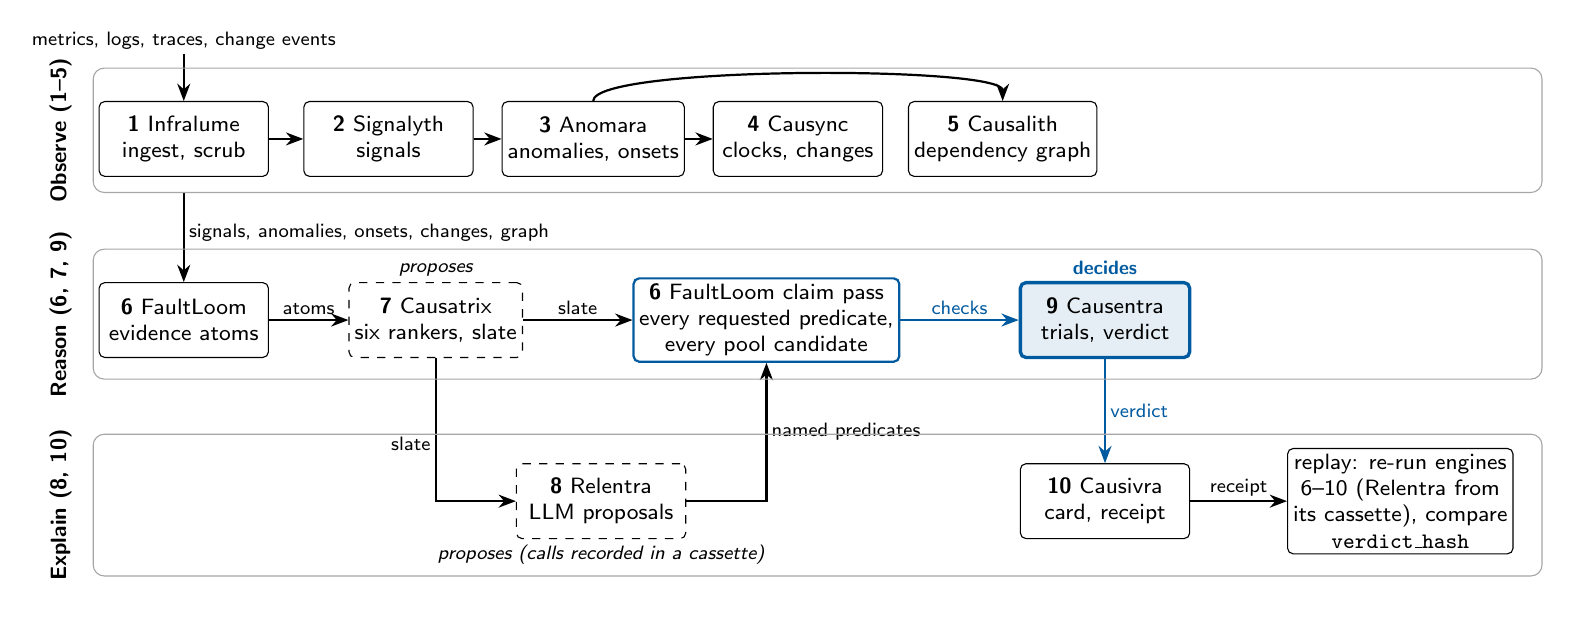
\begin{tikzpicture}[
  font=\sffamily\footnotesize,
  >={Stealth[length=2.2mm]},
  eng/.style={draw, rounded corners=2pt, minimum width=2.15cm, minimum height=0.95cm,
    align=center, inner sep=2pt, fill=white},
  prop/.style={eng, dashed},
  dec/.style={eng, draw=accent, very thick, fill=accent!10},
  code/.style={eng, draw=accent, thick},
  lane/.style={draw, gray!70, rounded corners=4pt},
  lanelabel/.style={font=\sffamily\footnotesize\bfseries, rotate=90, anchor=south},
  tag/.style={font=\sffamily\scriptsize\itshape, inner sep=1pt},
  lbl/.style={font=\sffamily\scriptsize, inner sep=1.5pt},
  flow/.style={->, thick},
]
% ---------------------------------------------------------------- Observe (1-5)
\node[eng] (in) at (0,0)    {\textbf{1} Infralume\\ingest, scrub};
\node[eng] (sg) at (2.6,0)  {\textbf{2} Signalyth\\signals};
\node[eng] (an) at (5.2,0)  {\textbf{3} Anomara\\anomalies, onsets};
\node[eng] (cs) at (7.8,0)  {\textbf{4} Causync\\clocks, changes};
\node[eng] (cl) at (10.4,0) {\textbf{5} Causalith\\dependency graph};
\draw[flow] (in) -- (sg);
\draw[flow] (sg) -- (an);
\draw[flow] (an) -- (cs);
% Causync and Causalith both follow Anomara and are independent of each other (docs/02 §4 step 4).
\draw[flow] (an.north) .. controls +(0,0.45) and +(0,0.45) .. (cl.north);
\node[lbl, above=0.6cm of in.north, anchor=south] (tel) {metrics, logs, traces, change events};
\draw[flow] (tel) -- (in);

% ---------------------------------------------------------------- Reason (6, 7, 9)
\node[eng]  (fl) at (0,-2.3)    {\textbf{6} FaultLoom\\evidence atoms};
\node[prop] (cx) at (3.2,-2.3)  {\textbf{7} Causatrix\\six rankers, slate};
\node[code, minimum width=3.3cm] (cp) at (7.4,-2.3) {\textbf{6} FaultLoom claim pass\\every requested predicate,\\every pool candidate};
\node[dec]  (ce) at (11.7,-2.3) {\textbf{9} Causentra\\trials, verdict};
\node[tag, above=1pt of cx.north] {proposes};
\node[tag, above=1pt of ce.north, text=accent] {\upshape\bfseries decides};
\draw[flow] (fl) -- node[lbl, above] {atoms} (cx);
\draw[flow] (cx) -- node[lbl, above] {slate} (cp);
\draw[flow, draw=accent] (cp) -- node[lbl, above, text=accent] {checks} (ce);
% Observe facts into FaultLoom
\draw[flow] (in.south |- 0,-0.68) -- node[lbl, right, pos=0.45] {signals, anomalies, onsets, changes, graph} (fl.north);

% ---------------------------------------------------------------- Explain (8, 10)
\node[prop] (rl) at (5.3,-4.6) {\textbf{8} Relentra\\LLM proposals};
\node[tag, below=1pt of rl.south] {proposes (calls recorded in a cassette)};
\node[eng]  (cv) at (11.7,-4.6) {\textbf{10} Causivra\\card, receipt};
\draw[flow] (cx.south) |- node[lbl, left, pos=0.3] {slate} (rl.west);
\draw[flow] (rl.east) -| node[lbl, right, pos=0.75] {named predicates} (cp.south);
\draw[flow, draw=accent] (ce) -- node[lbl, right, text=accent] {verdict} (cv);

% ---------------------------------------------------------------- receipt and replay
\node[eng, minimum width=2.6cm] (rp) at (15.45,-4.6) {replay: re-run engines\\6--10 (Relentra from\\its cassette), compare\\\texttt{verdict\_hash}};
\draw[flow] (cv) -- node[lbl, above] {receipt} (rp);

% ---------------------------------------------------------------- lane frames
\draw[lane] (-1.15,0.9) rectangle (17.25,-0.68);
\draw[lane] (-1.15,-1.4) rectangle (17.25,-3.05);
\draw[lane] (-1.15,-3.75) rectangle (17.25,-5.55);
\node[lanelabel] at (-1.3,0.11) {Observe (1--5)};
\node[lanelabel] at (-1.3,-2.225) {Reason (6, 7, 9)};
\node[lanelabel] at (-1.3,-4.65)  {Explain (8, 10)};
\end{tikzpicture}
\end{document}
